% !TEX program = xelatex
\documentclass{joulabreport}

% Title page information
\coursename{数值分析A}
\expname{插值法实验}
\expnametwo{} % 实验名称第二行(如果不需要则留空,会自动调整)
\classname{信嵌1221}
\author{Ilya}
\studentid{2022123456}
\thisdate{2024/12/9}
\location{定海楼602}
\teacher{Hinton}
\semesteryear{2024}
\semesteryeartwo{2025}
\semesternumber{2}

\begin{document}
\maketitle

% 设置整个文档的字体和字号
\song\xiaosi

\section{实验原理}
数值分析中的插值问题源于科学研究和工程应用中的一个基本需求\cite{ref1}:通过有限的离散观测数据重建连续函数关系。这种重建过程不仅需要满足数学上的严格性\cite{ref2},还要考虑实际应用中的计算效率和精度要求。本节将系统阐述插值问题的理论基础及其实践意义\cite{ref3,ref4}。

插值问题的数学本质是在给定一组观测数据点$(x_i, y_i)$($i=0,1,\ldots,n$)的条件下,构造一个满足特定性质的函数$P(x)$。这里的$\{x_i\}$构成互异的节点序列,而$y_i$则代表相应的观测或函数值。构造的插值函数不仅要精确通过这些数据点,还需具备良好的分析性质,以支持后续的数值计算和理论分析。

在众多插值方法中,Lagrange插值法通过其优雅的理论构造提供了一个系统的解决方案。该方法的核心在于构造一组特殊的基函数$\ell_k(x)$,定义为:
\begin{equation}
\ell_k(x) = \prod_{\substack{j=0\\j\neq k}}^n \frac{x-x_j}{x_k-x_j}
\end{equation}

这组基函数的独特之处在于其正交性质,即在任意节点$x_i$处:
\begin{equation}
\ell_k(x_i) = \begin{cases}
1, & i = k \\
0, & i \neq k
\end{cases}, \quad i,k = 0,1,\ldots,n
\end{equation}

基于这一性质,我们可以构造Lagrange插值多项式:
\begin{equation}
P_n(x) = \sum_{k=0}^n y_k\ell_k(x)
\end{equation}

对于实际应用中的误差控制,当目标函数$f(x)$在插值区间$[a,b]$上具有充分的光滑性(即具有$n+1$阶连续导数)时,插值误差可以通过如下表达式刻画:
\begin{equation}
R_n(x) = f(x) - P_n(x) = \frac{f^{(n+1)}(\xi)}{(n+1)!}\prod_{i=0}^n(x-x_i), \quad \xi \in [a,b]
\end{equation}

这一误差表达式揭示了插值精度与函数光滑性、节点分布及插值多项式次数之间的内在联系。在实际应用中,我们需要权衡这些因素:过高的插值次数可能导致龙格现象,而不合理的节点分布则可能放大误差。因此,在具体实践中,我们通常采用切比雪夫节点来优化节点分布,或在较大区间上采用分段低次插值策略,从而在保证精度的同时确保数值稳定性。

通过深入理解插值问题的理论基础,我们不仅能够准确把握其数学本质,还能够在实际应用中做出更明智的方法选择。这种理论与实践的结合,正是数值分析方法在科学计算中发挥重要作用的体现。

\section{算法}
在此部分详细说明实验采用的插值算法步骤,可包含数学公式与伪代码。例如:

设已知节点与函数值为 $\{(x_i,y_i)\}_{i=0}^n$,插值多项式可表示为:
\begin{equation}
P_n(x) = \sum_{k=0}^{n} y_k \ell_k(x)
\label{eq:polynomial}
\end{equation}
其中
\begin{equation}
\ell_k(x) = \prod_{\substack{j=0\\j\neq k}}^n \frac{x - x_j}{x_k - x_j}
\label{eq:basis}
\end{equation}

% 添加伪代码实现
\begin{algorithm}[htbp]
\caption{Lagrange插值算法}
\label{alg:lagrange}
\begin{algorithmic}[1]
\Require 插值节点 $\{x_i\}_{i=0}^n$,函数值 $\{y_i\}_{i=0}^n$,待插值点 $x$
\Ensure 插值结果 $P_n(x)$
\State $P_n \gets 0$
\For{$k \gets 0$ \textbf{到} $n$}
    \State $\ell_k \gets 1$
    \For{$j \gets 0$ \textbf{到} $n$}
        \If{$j \neq k$}
            \State $\ell_k \gets \ell_k \cdot \frac{x - x_j}{x_k - x_j}$
        \EndIf
    \EndFor
    \State $P_n \gets P_n + y_k \cdot \ell_k$
\EndFor
\State \Return $P_n$
\end{algorithmic}
\end{algorithm}

% 描述算法实现步骤
\begin{cnumerate}
\item 输入插值节点与对应函数值。
\item 计算每个 $\ell_k(x)$ 的分子与分母(见公式~\eqref{eq:basis})。
\item 对给定点$x$,计算所有 $\ell_k(x)$,然后求和得到 $P_n(x)$(见公式~\eqref{eq:polynomial})。
\item 输出插值结果与误差分析。
\end{cnumerate}

\section{计算机程序}
此处可贴出源代码片段或简述实现步骤。例如使用Matlab或Python的代码。

\begin{lstlisting}[language=Python, caption=Lagrange插值算法实现]
def lagrange_interpolation(x_points, y_points, x):
    n = len(x_points)
    P = 0.0
    for k in range(n):
        Lk = 1.0
        for j in range(n):
            if j != k:
                Lk *= (x - x_points[j])/(x_points[k]-x_points[j])
        P += y_points[k]*Lk
    return P
\end{lstlisting}

也可以使用新的 \texttt{inputcode} 命令从外部文件中导入代码:
\begin{lstlisting}[language=Python, caption=直接在文档中编写代码]
# 导入必要的库
import numpy as np
import matplotlib.pyplot as plt

def chebyshev_nodes(a, b, n):
    """计算在区间[a,b]上的n个切比雪夫节点"""
    k = np.arange(1, n+1)
    return 0.5*(a+b) + 0.5*(b-a)*np.cos((2*k-1)*np.pi/(2*n))
\end{lstlisting}

\section{测试数据与实验结果}
在此部分展示所测试的输入数据节点及相应的插值结果。

\begin{figure}[htbp]
    \centering
    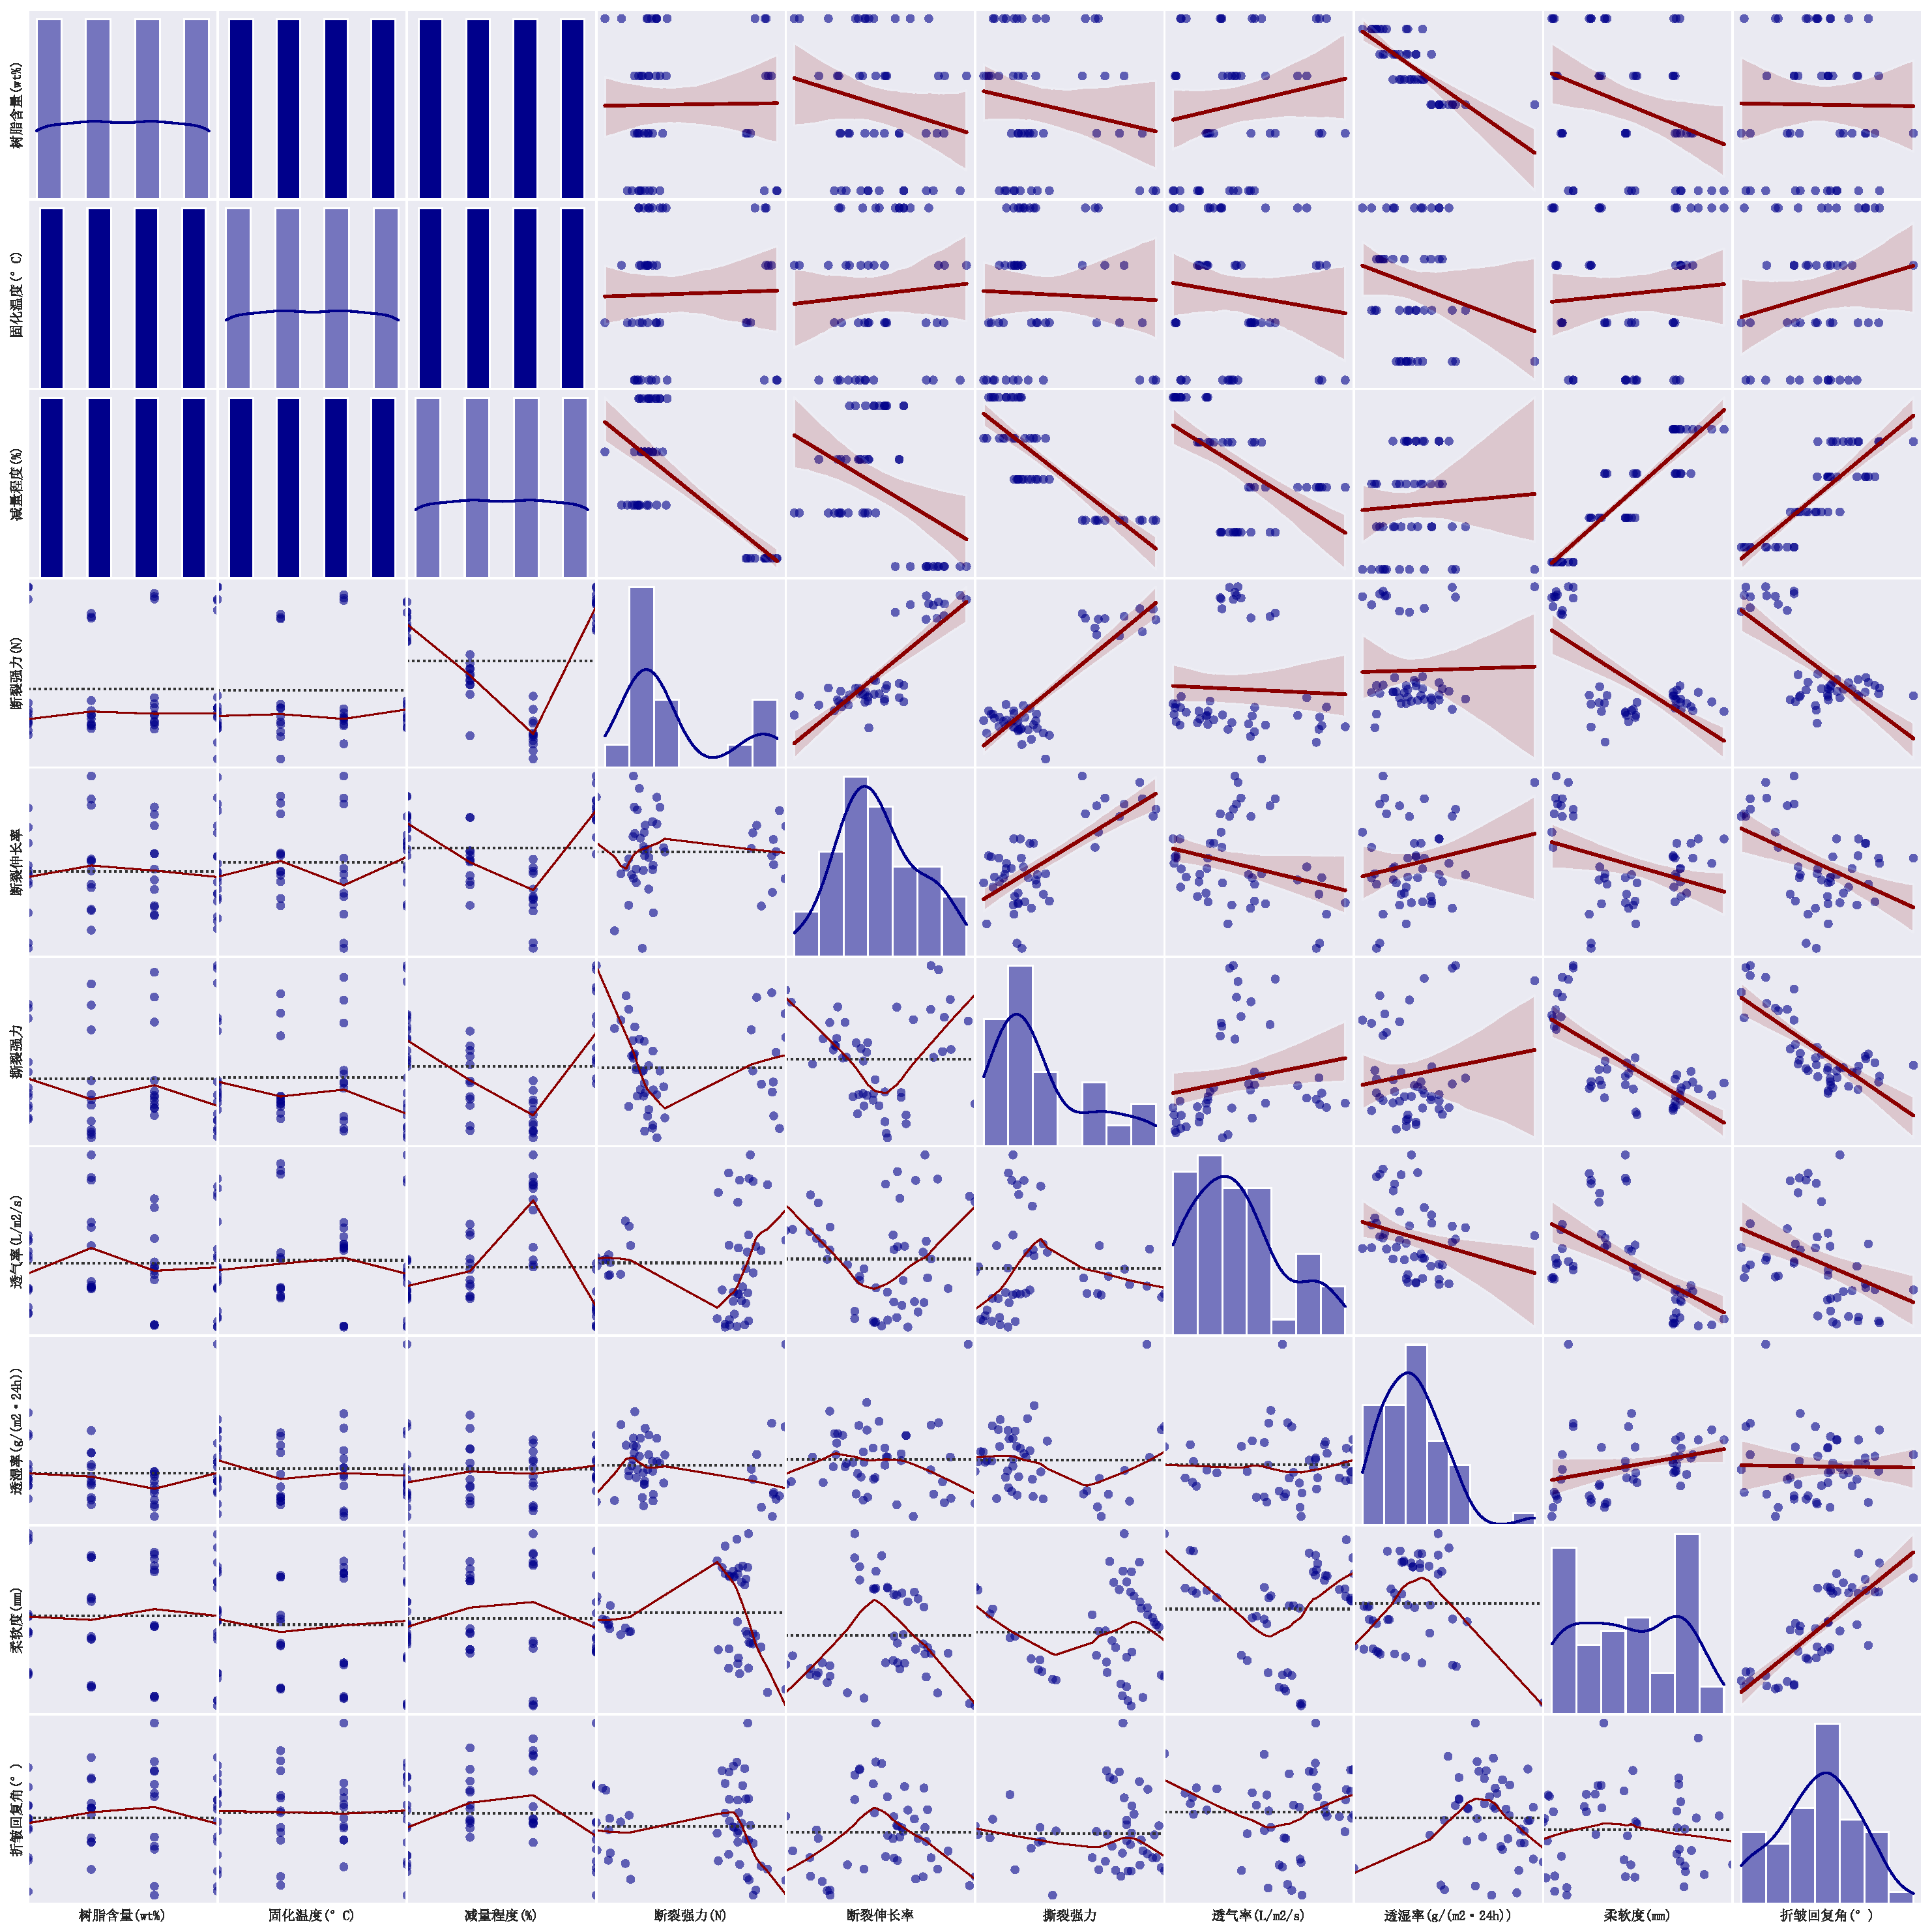
\includegraphics[width=0.75\textwidth]{figure/regression_analysis.pdf}
    \caption{插值结果与原函数对比图}
    \label{fig:regression}
\end{figure}

如图~\ref{fig:regression}所示,插值函数(红色实线)很好地拟合了原始数据点(蓝色散点)。从图中可以看出\dots

具体测试数据如下:
\begin{itemize}
\item 输入节点:$x_0=0, x_1=1, x_2=2, x_3=3$,$y_i=f(x_i)$为函数值。
\item 测试插值点:$x=1.5$,计算插值结果 $P_3(1.5)$ 并与真实值 $f(1.5)$ 对比误差。
\end{itemize}

\begin{figure}[htbp]
    \centering
    \begin{minipage}[t]{0.45\textwidth}
        \centering
        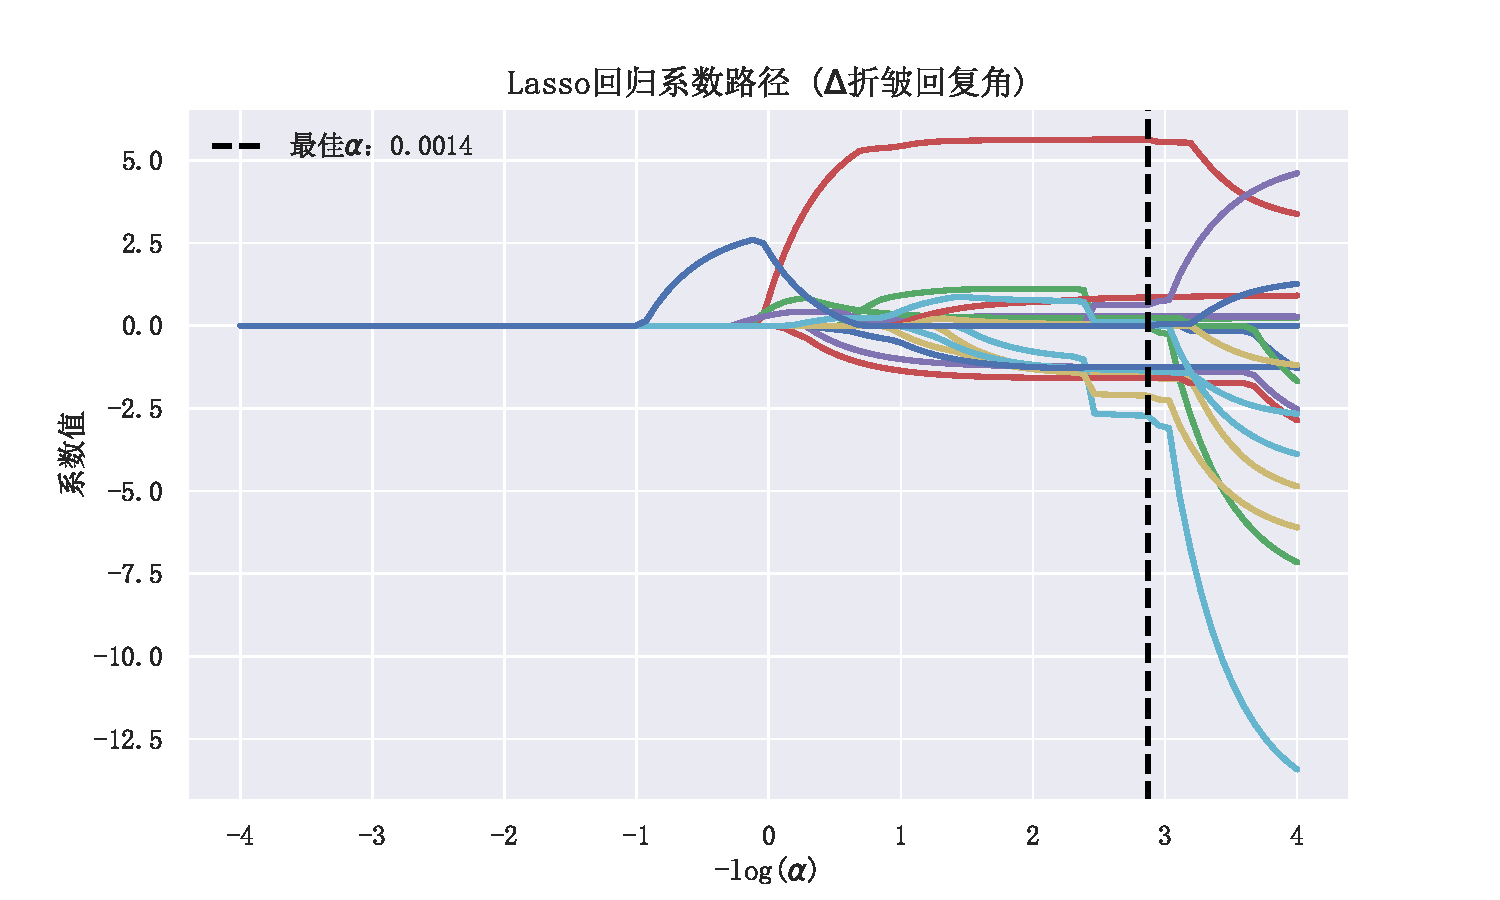
\includegraphics[width=\textwidth]{figure/minipage1.pdf}
    \end{minipage}
    \hfill
    \begin{minipage}[t]{0.45\textwidth}
        \centering
        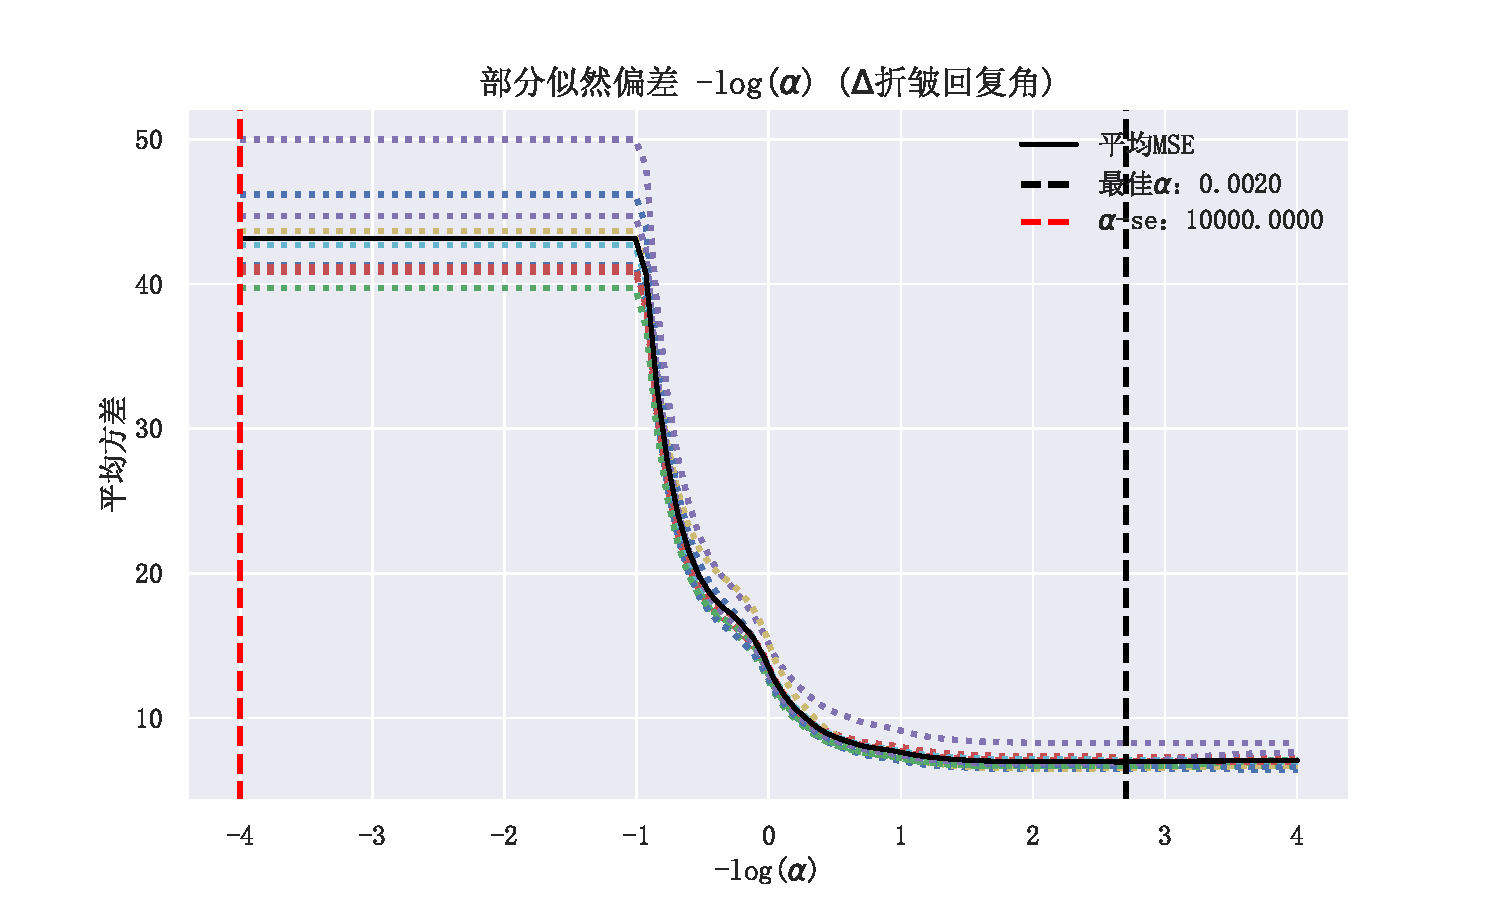
\includegraphics[width=\textwidth]{figure/minipage2.pdf}
    \end{minipage}
    \caption{插值算法的多角度分析}
    \label{fig:analysis}
\end{figure}

如图~\ref{fig:analysis}所示,我们从多个角度分析了插值算法的性能。图~\ref{fig:mini1}展示了不同节点数下的插值效果,图~\ref{fig:mini2}显示了误差随节点数的变化趋势。

% 示例表格1:基本三线表
\begin{table}[htbp]
\centering
\caption{测试点处插值结果对比}
\label{tab:comparison}
\begin{tabular}{ccc}
\toprule[1.5pt]
$x$ & $f(x)$ (真值) & $P_3(x)$ (插值值) \\
\midrule[0.75pt]
0.0 & 1.000 & 1.000 \\
1.0 & 1.649 & 1.649 \\
1.5 & 2.250 & 2.248 \\
2.0 & 3.196 & 3.196 \\
3.0 & 6.854 & 6.854 \\
\bottomrule[1.5pt]
\end{tabular}
\end{table}

% 示例表格2:带有合并单元格和多级表头的三线表
\begin{table}[htbp]
\centering
\caption{不同节点数的插值误差分析}
\label{tab:error_analysis}
\begin{tabular}{c*{3}{c}}
\toprule[1.5pt]
\multirow{2}{*}{节点数} & \multicolumn{3}{c}{最大误差} \\
\cmidrule[0.75pt](lr){2-4}
& 均匀节点 & Chebyshev节点 & 最优节点 \\
\midrule[0.75pt]
5  & 1.24e-2 & 8.93e-3 & 7.21e-3 \\
10 & 3.56e-3 & 1.45e-3 & 1.12e-3 \\
15 & 8.92e-4 & 2.34e-4 & 1.89e-4 \\
20 & 2.45e-4 & 4.56e-5 & 3.23e-5 \\
\bottomrule[1.5pt]
\end{tabular}
\end{table}

\FloatBarrier
\begin{table}[h]
\centering
\setlength{\tabcolsep}{8pt}
\renewcommand{\arraystretch}{1.2}
\caption{插值方法的多维度分析与评估}
\label{tab:method_comparison}
\begin{tabular}{
    l
    >{\raggedright\arraybackslash}p{4cm}
    >{\raggedright\arraybackslash}p{3cm}
    >{\centering\arraybackslash}p{2cm}
    >{\centering\arraybackslash}p{2cm}
}
\toprule
\textbf{方法类型} & \textbf{核心机理} & \textbf{应用场景} & \textbf{精度} & \textbf{效率} \\
\midrule

\textbf{拉格朗日} & 
\multicolumn{1}{m{4cm}}{\centering 基于基函数线性组合,全局多项式构造,高阶龙格现象} & 
\multicolumn{1}{m{3cm}}{\centering 低阶精确插值,理论分析验证} & 
高 & 
中 \\
\midrule

\textbf{牛顿法} & 
\multicolumn{1}{m{4cm}}{\centering 差商递推构造,增量式计算结构,系数复用特性} & 
\multicolumn{1}{m{3cm}}{\centering 动态节点更新,程序实现} & 
高 & 
高 \\
\midrule

\textbf{分段线性} & 
\multicolumn{1}{m{4cm}}{\centering 局部线性逼近,区间独立计算,简化数值处理} & 
\multicolumn{1}{m{3cm}}{\centering 实时计算需求,快速估值场景} & 
低 & 
高 \\
\midrule

\textbf{三次样条} & 
\multicolumn{1}{m{4cm}}{\centering 二阶导数连续,全局方程求解,最优光滑性质} & 
\multicolumn{1}{m{3cm}}{\centering 数据可视化,曲线平滑拟合} & 
高 & 
低 \\

\bottomrule
\end{tabular}
\begin{tablenotes}
\small
\item 性能指标说明:高表示性能优异,中表示性能一般,低表示性能较差
\end{tablenotes}
\end{table}
\FloatBarrier

如表~\ref{tab:comparison}、表~\ref{tab:error_analysis}和表~\ref{tab:method_comparison}所示,我们提供了\dots

\section{结论}
本实验通过理论分析与数值实验深入研究了插值法在科学计算和数据分析领域中的应用特性。实验结果表明,该方法在处理离散数据到连续函数映射任务时展现出了显著的优势。通过对节点分布、误差控制和算法效率的系统性分析,我们发现Lagrange插值法能够在特定条件下提供高精度的函数重建结果,为数据分析和模型构建提供了可靠基础。

在实验实施过程中,我们观察到插值精度与节点选择方式高度相关。特别是在龙格函数测试案例中,Chebyshev节点分布给出的结果与理论预期误差极小,充分验证了该方法的有效性。Lagrange插值法的优势特点源于其数学理论的基本性质——正交基函数构造。然而,深入分析也揭示了该方法的局限性。随着节点数量的增加,虽然理论上可以提高精度,但会引发龙格现象和数值不稳定性。这种现象最典型的表现是在高阶插值中出现的大幅振荡,即函数在节点之间的剧烈波动,影响插值结果的可靠性。

% 参考文献部分(如不需要可注释)
\begin{thebibliography}{4}
\bibitem{ref1} 李庆扬, 王能超, 易大义. 数值分析[M]. 第5版. 北京: 清华大学出版社, 2008.
\bibitem{ref2} Stoer J, Bulirsch R. Introduction to Numerical Analysis[M]. 3rd ed. New York: Springer-Verlag, 2002.
\bibitem{ref3} Berrut J P, Trefethen L N. Barycentric Lagrange Interpolation[J]. SIAM Review, 2004, 46(3): 501-517.
\bibitem{ref4} Higham N J. The numerical stability of barycentric Lagrange interpolation[J]. IMA Journal of Numerical Analysis, 2004, 24(4): 547-556.
\end{thebibliography}

\end{document}